% !TEX root = A0.MiTFG.tex

\chapter{Implementación}

Este capítulo describe la materialización de la arquitectura propuesta en Fase~1 y Fase~2. Ambas reutilizan el activo Widevine y los servicios de medios del entorno experimental, pero modifican de forma sustancial el camino de acceso: Varnish dirige las operaciones al \textit{control-plane}, el origen y el servidor de licencias dejan de publicarse en el anfitrión y el cliente necesita una sesión activa para cargar el manifiesto, recuperar contenido local o solicitar una licencia.

La exposición se centra en decisiones comprobables en el código y en la configuración desplegada. Los valores indicados corresponden al prototipo ejecutado; no se presentan como parámetros universales para un servicio OTT. Las pruebas comparativas, los códigos observados y el impacto de los controles se han desarrollado en el Capítulo~7.

\section{Despliegue con Docker}

\subsection{Contenedores}

Fase~1 se despliega mediante siete contenedores: Varnish, \textit{control-plane}, origen Nginx, servidor interno de licencias, cliente OTT, laboratorio de auditoría y laboratorio de CDN leeching. Fase~2 conserva esos componentes y añade Redis, alcanzando ocho servicios. El cliente y el laboratorio general son aplicaciones estáticas servidas por Nginx; el plano de control, el proxy de licencia y el laboratorio de CDN leeching se implementan con Node.js y Express.

\begin{table}[H]
\centering
\caption{Contenedores de las fases endurecidas}
\label{tab:contenedores-fases}
\begin{tabularx}{\textwidth}{p{0.22\textwidth}Yp{0.15\textwidth}}
\toprule
\textbf{Servicio} & \textbf{Función implementada} & \textbf{Fases} \\
\midrule
\texttt{cdn} & Frontal Varnish, lista de rutas, CORS, normalización de IP y derivación al plano de control. & 1 y 2 \\
\texttt{control-plane} & Login, autorización, sesiones, tokens, manifiesto, contenido, licencia y, en Fase~2, riesgo y administración. & 1 y 2 \\
\texttt{origin} & Publicación interna y de solo lectura del árbol \texttt{origin-content}. & 1 y 2 \\
\texttt{license-server} & Proxy interno del challenge hacia el servicio Widevine de pruebas. & 1 y 2 \\
\texttt{ott-client} & Cliente oficial con Shaka Player, watermark y controles de sesión. & 1 y 2 \\
\texttt{audit-lab} & Reproducción controlada, inspección de atributos y escenarios reproducibles. & 1 y 2 \\
\texttt{key-leak-lab} & Cliente externo controlado para Key Leak, CORS, concurrencia y reutilización contextual. & 1 y 2 \\
\texttt{redis} & Sesiones, eventos, riesgo, contadores y bans sin persistencia en disco. & 2 \\
\bottomrule
\end{tabularx}
\end{table}

Las imágenes de Nginx y Redis proceden de versiones ligeras basadas en Alpine. Varnish utiliza la imagen 7.5 y reserva 256~MB para su almacenamiento en memoria. Los servicios Node.js se construyen desde los directorios correspondientes, lo que permite modificar su lógica sin mezclarla con la imagen de distribución.

\subsection{Redes}

Cada fase define una red Docker independiente: \texttt{tfm-fase1-net} y \texttt{tfm-fase2-net}. Los nombres de servicio actúan como resolución interna, de modo que el \textit{control-plane} alcanza \texttt{http://origin} y \texttt{http://license-server:8080} sin publicar esos puertos. En Fase~2, Redis solo escucha dentro de la misma red como \texttt{redis:6379}.

La ausencia de puertos del anfitrión para origen y licencia corrige la ruta directa observada en Fase~0. No se trata únicamente de ocultar direcciones: Varnish remite todas las operaciones públicas al \textit{control-plane}, que vuelve a aplicar la política antes de acceder a los servicios internos. Los activos compartidos se montan en Nginx como volumen de solo lectura.

\subsection{Servicios y puertos}

La Tabla~\ref{tab:puertos-fases} recoge las interfaces publicadas. Los puertos de cliente y laboratorio se separan para que las acciones de auditoría no tengan que incorporarse a la aplicación oficial.

\begin{table}[H]
\centering
\caption{Interfaces publicadas en el anfitrión}
\label{tab:puertos-fases}
\begin{tabularx}{\textwidth}{p{0.11\textwidth}p{0.17\textwidth}p{0.18\textwidth}p{0.20\textwidth}Y}
\toprule
\textbf{Fase} & \textbf{Cliente} & \textbf{Lab. auditoría} & \textbf{Lab. CDN leeching} & \textbf{CDN / API} \\
\midrule
Fase~1 & \texttt{localhost:9300} & \texttt{localhost:9301} & \texttt{localhost:9302} & \texttt{localhost:9080} \\
Fase~2 & \texttt{localhost:9400} & \texttt{localhost:9401} & \texttt{localhost:9402} & \texttt{localhost:9180} \\
\bottomrule
\end{tabularx}
\end{table}

El \textit{control-plane}, el origen, el servidor de licencias y Redis no se publican directamente. Los secretos HMAC y las credenciales de los dos usuarios se suministran como valores de demostración. Al igual que el uso de HTTP local, esta configuración facilita la reproducción del laboratorio, pero debería sustituirse por TLS, gestión de secretos e identidad externa en un despliegue real.

\section{Desarrollo del plano de control y del proxy protegido}

\subsection{Arquitectura software}

El \textit{control-plane} es una aplicación Express que combina tres responsabilidades acotadas. La primera es emitir y verificar credenciales. La segunda es mantener el ciclo de vida de las sesiones. La tercera es actuar como proxy autorizado hacia el manifiesto, el origen local y el servidor interno de licencias. Fase~1 conserva sesiones y límites en estructuras \texttt{Map} del proceso; Fase~2 reemplaza el estado operativo por claves y estructuras de Redis.

El manifiesto Widevine se obtiene desde la URL pública de Sintel únicamente después de validar la reproducción. El servicio inserta un elemento \texttt{BaseURL} con el directorio externo de los medios y devuelve el MPD como \texttt{application/dash+xml}. Esta reescritura permite que Shaka resuelva correctamente los segmentos aunque el MPD se haya solicitado a la URL local protegida. En consecuencia, el control implementado gobierna la entrega del manifiesto y el inicio del flujo; los segmentos del activo público continúan alojados fuera del laboratorio.

Para el contenido local, el manifiesto CENC se obtiene del origen, se normaliza como una presentación estática de 60~s y se reescribe para que cada \texttt{BaseURL} apunte a \texttt{/content/dash-known-key/}. Esta ruta elimina el prefijo público, contrasta la ruta con el activo del token y solo entonces reenvía la solicitud a Nginx. La respuesta conserva cabeceras como \texttt{Content-Type}, \texttt{Content-Length}, rangos y ETag. El mapeo explícito impide usar un token de un activo para recorrer otro prefijo del origen y obliga a autorizar también las inicializaciones y los segmentos.

La licencia sigue una cadena diferente. Express recibe el cuerpo binario con un límite de 2~MB, valida la sesión y envía el challenge a \texttt{/internal/license}. La llamada interna añade cuenta, dispositivo, activo y sesión como cabeceras. El servidor de licencias exige la presencia de ese contexto antes de reenviar el cuerpo al servicio CWIP de pruebas y marca la respuesta como no cacheable.

\subsection{\textit{Endpoints}}

La interfaz HTTP se mantiene prácticamente igual entre las fases. Fase~2 añade los endpoints administrativos y eventos asociados. La Tabla~\ref{tab:endpoints-fases} resume el contrato implementado.

\begin{table}[H]
\centering
\caption{Endpoints principales de Fase~1 y Fase~2}
\label{tab:endpoints-fases}
\begin{tabularx}{\textwidth}{p{0.13\textwidth}p{0.30\textwidth}Yp{0.12\textwidth}}
\toprule
\textbf{Método} & \textbf{Ruta} & \textbf{Credencial y función} & \textbf{Fases} \\
\midrule
GET & \texttt{/health} & Estado del servicio y sesiones conocidas. & 1 y 2 \\
POST & \texttt{/auth/login} & Credenciales de usuario; emite el token de acceso. & 1 y 2 \\
POST & \texttt{/playback/session} & Token de acceso; valida entitlement y concurrencia. & 1 y 2 \\
GET & \texttt{/manifest/:assetId} & Token de reproducción; entrega el MPD asociado. & 1 y 2 \\
GET/HEAD & \texttt{/content/*} & Token de reproducción; proxy al prefijo local autorizado. & 1 y 2 \\
POST & \texttt{/license} & Token de reproducción; proxy del challenge Widevine. & 1 y 2 \\
POST & \texttt{/playback/heartbeat} & Token de reproducción; mantiene sesión y rota token. & 1 y 2 \\
POST & \texttt{/playback/stop} & Token de reproducción; detiene la sesión. & 1 y 2 \\
GET & \texttt{/admin/overview} & Token de acceso con rol admin; resumen operativo. & 2 \\
GET & \texttt{/admin/events} & Token de acceso con rol admin; eventos recientes. & 2 \\
POST & \texttt{/admin/bans} & Crea un ban de cuenta o dispositivo. & 2 \\
POST & \texttt{/admin/bans/clear} & Retira un ban existente. & 2 \\
\bottomrule
\end{tabularx}
\end{table}

La ruta heredada \texttt{/license/no\_auth} no aparece en la lista permitida de Varnish ni existe en Express. De esta forma no hay un segundo camino público que evite las comprobaciones del endpoint protegido.

\subsection{\textit{Middleware} y perímetro}

Varnish responde a las preflight CORS y solo admite los orígenes de cliente y laboratorio de su fase. Las cabeceras autorizadas se limitan a autorización, tipo de contenido, rangos, sesión, dispositivo e instancia de cliente. En Fase~2 se expone además \texttt{X-Risk-Score}. Todas las respuestas del frontal se marcan como \texttt{no-store}, puesto que el prototipo prioriza la consistencia de las decisiones sobre una evaluación de caché. CORS limita un reproductor ejecutado desde un origen web ajeno, pero no autentica un cliente nativo o un backend; estos siguen dependiendo de la validación del token.

Antes de enviar la petición al backend, Varnish comprueba que la ruta pertenezca al conjunto esperado y exige \texttt{Authorization} en las operaciones protegidas. Sobrescribe \texttt{X-Forwarded-For} con la IP de la conexión, añade \texttt{X-Request-Id} y fuerza el paso directo al backend. Express aplica a continuación la comprobación criptográfica y contextual; por tanto, la presencia de la cabecera en Varnish no se considera prueba suficiente de autorización.

\section{Implementación de validaciones}

\subsection{Credenciales de acceso y reproducción}

Las credenciales se serializan y firman localmente. Antes de interpretar sus atributos, el servidor comprueba su integridad y rechaza cualquier valor alterado.

La credencial de acceso identifica la cuenta, el dispositivo y sus permisos; la de reproducción incorpora el activo, la sesión, la instancia de cliente y las operaciones permitidas. Ambas utilizan secretos distintos para impedir que una credencial de acceso pueda aceptarse como autorización de reproducción.

La Tabla~\ref{tab:parametros-sesion} muestra los parámetros comunes configurados en Docker Compose.

\begin{table}[H]
\centering
\caption{Parámetros de credenciales y sesiones}
\label{tab:parametros-sesion}
\begin{tabularx}{\textwidth}{Yp{0.22\textwidth}p{0.30\textwidth}}
\toprule
\textbf{Parámetro} & \textbf{Valor} & \textbf{Finalidad} \\
\midrule
Expiración del token de acceso & 3600~s & Mantener la identidad de la sesión de usuario. \\
Expiración del token de reproducción & 90~s & Reducir la ventana de reutilización. \\
Gracia de heartbeat & 45~s & Expirar sesiones que dejan de mantenerse. \\
Periodo del heartbeat del cliente & 20~s & Renovar antes de la expiración o la gracia. \\
Máximo de sesiones activas & 1 por cuenta & Reproducir el control de concurrencia. \\
Retención de eventos en Fase~2 & 300 eventos & Acotar el estado de observabilidad. \\
Umbral de auto-ban de cuenta & 100 puntos & Activar respuesta por riesgo acumulado. \\
\bottomrule
\end{tabularx}
\end{table}

\subsection{Validación de IP, dispositivo, instancia, activo y sesión}

La implementación no realiza geolocalización. La IP fiable proporcionada por Varnish se utiliza para rate limiting en Fase~1 y para correlación temporal en Fase~2. El \texttt{deviceId} se genera en el navegador y se incluye en el login. Al crear la reproducción se genera también un \texttt{clientInstanceId}, que queda ligado al token y a la sesión. Cada validación compara cuenta, dispositivo, instancia y activo del token con el objeto de sesión almacenado.

El manifiesto contrasta también el \texttt{assetId} de la ruta, mientras que manifiesto, contenido y licencia comparan las cabeceras \texttt{X-Playback-Session-Id} y \texttt{X-Client-Instance-Id}. Un activo diferente se rechaza como falta de autorización, una sesión diferente como conflicto y una instancia copiada como credencial no válida. Esta distinción facilita el análisis posterior sin revelar el token utilizado.

Fase~2 ejecuta además la comprobación de bans en las operaciones que emplean credenciales de acceso o reproducción. El plano administrativo usa una validación separada de rol. Esta separación es intencional: un operador debe poder consultar y retirar un ban aunque su dispositivo no pueda utilizar el plano de reproducción.

\subsection{Control de sesiones, concurrencia y expiración}

La creación de sesión elimina primero las sesiones que han superado la gracia de heartbeat. Después comprueba el entitlement, exige la instancia de cliente y cuenta las sesiones activas de la cuenta. Si no se supera el máximo, genera un UUID, almacena el contexto y emite el token de reproducción.

Fase~1 guarda los objetos en memoria. Fase~2 emplea claves \texttt{session:<uuid>} y un conjunto \texttt{account-sessions:<accountId>}. Las sesiones tienen un TTL operativo de 900~s y el índice por cuenta, de 24 horas. El proceso revisa cada diez segundos las sesiones conocidas y marca como \texttt{expired} las que superan los 45~s sin heartbeat. La parada explícita utiliza el estado \texttt{stopped}.

El cliente llama al heartbeat cada 20~s. La respuesta contiene un nuevo token de reproducción de 90~s, por lo que la rotación se realiza antes de la expiración. La renovación no cambia el identificador de sesión ni el activo y vuelve a comprobar el estado almacenado.

Fase~1 incorpora además límites en memoria por IP y minuto: 20 intentos de autenticación, 60 creaciones de sesión, 120 manifiestos, 180 heartbeats, 600 solicitudes de contenido y 120 licencias. Fase~2 no replica este limitador duro como módulo independiente; utiliza contadores persistentes para elevar riesgo y terminar en bloqueo. Esta diferencia se conserva expresamente en la descripción para no afirmar que ambas fases aplican exactamente la misma semántica de rate limiting.

\section{Sistema de \textit{logging} y monitorización}

Fase~2 registra cada evento como JSON en una lista Redis limitada a 300 elementos. El productor añade UUID, tipo y marca temporal a los campos específicos de la operación. Entre los tipos implementados se encuentran \texttt{auth.success}, \texttt{auth.failure}, \texttt{auth.blocked}, \texttt{playback.session\_created}, \texttt{playback.concurrency\_rejected}, \texttt{playback.client\_instance\_rejected}, \texttt{manifest.request}, \texttt{content.request}, \texttt{license.request}, \texttt{key\_leak.pattern\_detected}, \texttt{playback.heartbeat}, \texttt{playback.stopped}, \texttt{playback.expired}, \texttt{risk.incremented}, \texttt{ban.created} y \texttt{ban.cleared}.

La puntuación de riesgo se almacena durante 24 horas junto con un máximo de ocho razones distintas. Un login desde menos de tres IP recientes reduce cinco puntos, mientras que los patrones de la Tabla~\ref{tab:reglas-riesgo} incrementan el valor o crean un ban directo.

\begin{table}[H]
\centering
\caption{Reglas implementadas en Fase~2}
\label{tab:reglas-riesgo}
\begin{tabularx}{\textwidth}{Yp{0.22\textwidth}p{0.25\textwidth}}
\toprule
\textbf{Señal} & \textbf{Ventana / umbral} & \textbf{Acción} \\
\midrule
Actividad multi-IP & 3 IP en 10~min & $+30$ puntos de cuenta \\
Concurrencia rechazada & 2 en 10~min & $+25$ puntos \\
Solicitudes de licencia & 6 en 5~min & $+20$ puntos \\
Solicitudes de contenido & 40 en 1~min & $+15$ puntos \\
Contenido sin licencia & 3 objetos tras el manifest, una vez por sesión & $+20$ puntos \\
Heartbeats & 8 en 1~min & $+10$ puntos \\
Fallos de autenticación & 8 en 5~min & Ban de dispositivo de 15~min \\
Riesgo acumulado & $\geq 100$ puntos & Ban de cuenta de 30~min \\
\bottomrule
\end{tabularx}
\end{table}

Los contadores utilizan TTL y se incrementan de forma atómica en Redis. Los bans se guardan como \texttt{ban:account:<id>} o \texttt{ban:device:<id>} e incluyen razón, creador y expiración. La API administrativa permite crear bans con una duración indicada, listar el estado relevante para la cuenta autenticada y retirar un bloqueo.

El panel de Fase~2 representa los eventos mediante nodos de texto, no mediante HTML interpretado. Además, las interfaces muestran identificadores abreviados y atributos seleccionados, pero no imprimen \texttt{accessToken} ni \texttt{playbackToken} completos. Estas decisiones evitan que la propia instrumentación exponga credenciales reutilizables.

\section{Clientes y laboratorios de auditoría}

Los clientes oficiales mantienen separado el flujo de usuario de las acciones de auditoría. En ambos casos, el usuario autorizado inicia sesión, crea una reproducción y deja que Shaka Player añada el token y la instancia a las solicitudes de manifiesto, contenido local y licencia. Un watermark superpuesto utiliza correo enmascarado, prefijo de sesión y fase; aporta atribución visual, pero no se considera una medida criptográfica.

El laboratorio de Fase~1 automatiza login, creación de sesión y obtención del token a partir de usuario y contraseña. Muestra únicamente tipo, activo, expiración y scopes decodificados. También permite reproducir y ejecutar cuatro casos negativos: ausencia de token, token alterado, sesión distinta y activo distinto. La Figura~\ref{fig:fase1-cliente-laboratorio} presenta en paralelo el cliente legítimo y el laboratorio, ambos utilizando las mismas rutas protegidas.

\begin{figure}[htbp]
    \centering
    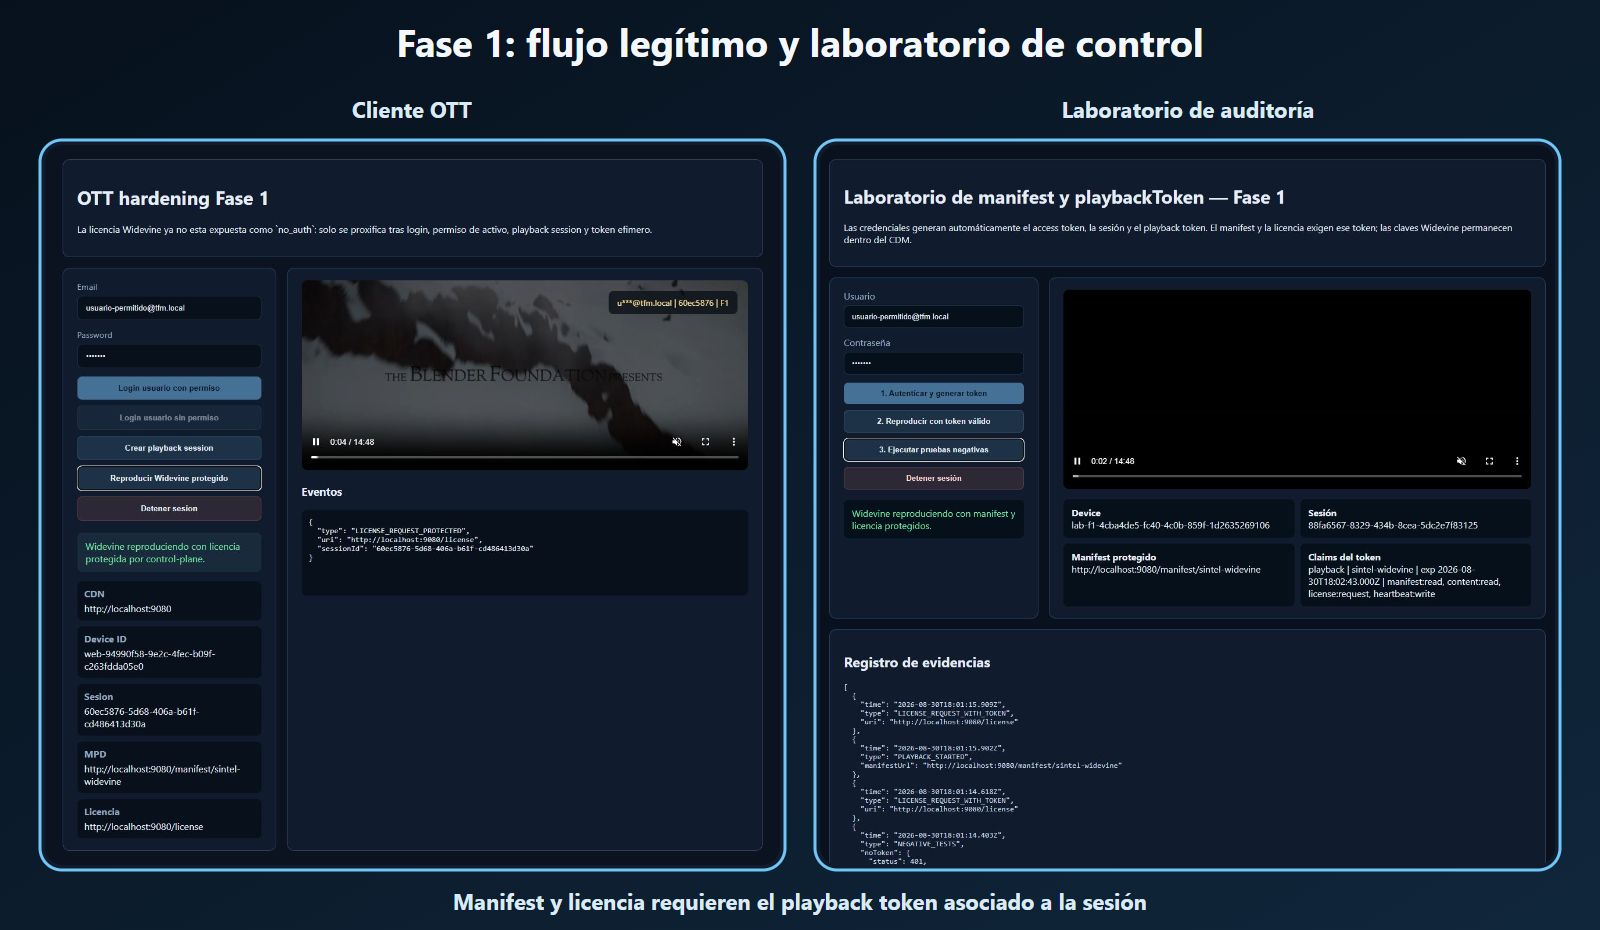
\includegraphics[width=0.98\textwidth]{figuras/fase1-cliente-laboratorio.png}
    \caption{Cliente oficial y laboratorio de Fase~1 utilizando manifiesto y licencia protegidos.}
    \label{fig:fase1-cliente-laboratorio}
\end{figure}

El cliente de Fase~2 añade un panel de observabilidad que consulta \texttt{/admin/overview}. La respuesta integra sesiones, score, razones, bans y los veinte eventos más recientes. Los botones administrativos crean o retiran un ban del dispositivo visible. La Figura~\ref{fig:fase2-cliente-observabilidad} muestra la reproducción legítima y la aparición de eventos de sesión, manifiesto y licencia; su análisis cuantitativo se presenta en el capítulo de evaluación.

\begin{figure}[htbp]
    \centering
    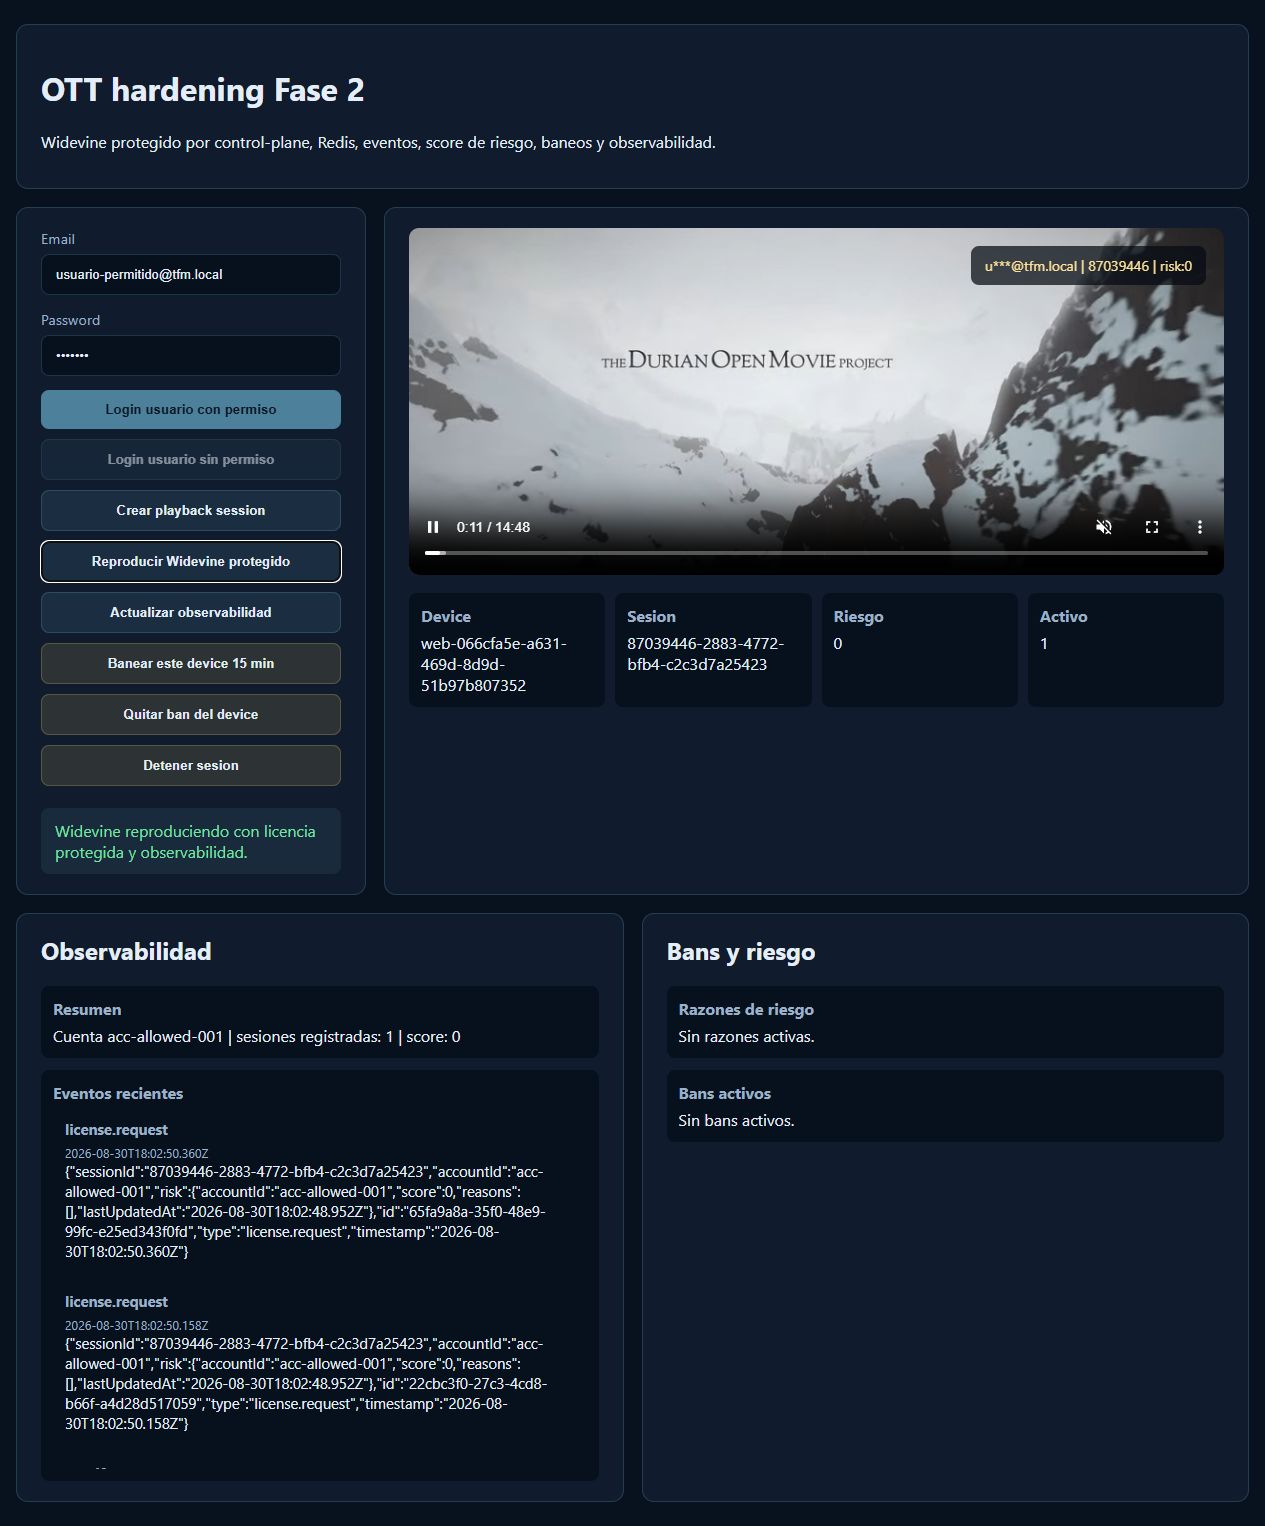
\includegraphics[height=0.82\textheight]{figuras/fase2-cliente-observabilidad.png}
    \caption{Cliente de Fase~2 con reproducción activa y panel de observabilidad.}
    \label{fig:fase2-cliente-observabilidad}
\end{figure}

El laboratorio de Fase~2 conserva las pruebas del manifiesto y añade dos secuencias de bloqueo reproducibles. La primera envía ocho logins con contraseña incorrecta y el mismo \texttt{deviceId}, lo que activa el ban temporal de dispositivo. La segunda mantiene una sesión legítima y solicita cinco sesiones adicionales: todas reciben \texttt{409 CONCURRENCY\_LIMIT}; el score observado progresa como 0, 25, 50, 75 y 100, y se activa el ban de cuenta. En ambos casos se detiene el heartbeat, se descarga el reproductor y se vuelve a solicitar el manifiesto con el token existente. La Figura~\ref{fig:fase2-laboratorio-bloqueo} documenta el segundo escenario: además del estado visible, el registro local conserva la progresión, el motivo del ban y el rechazo \texttt{401} del manifiesto.

\begin{figure}[htbp]
    \centering
    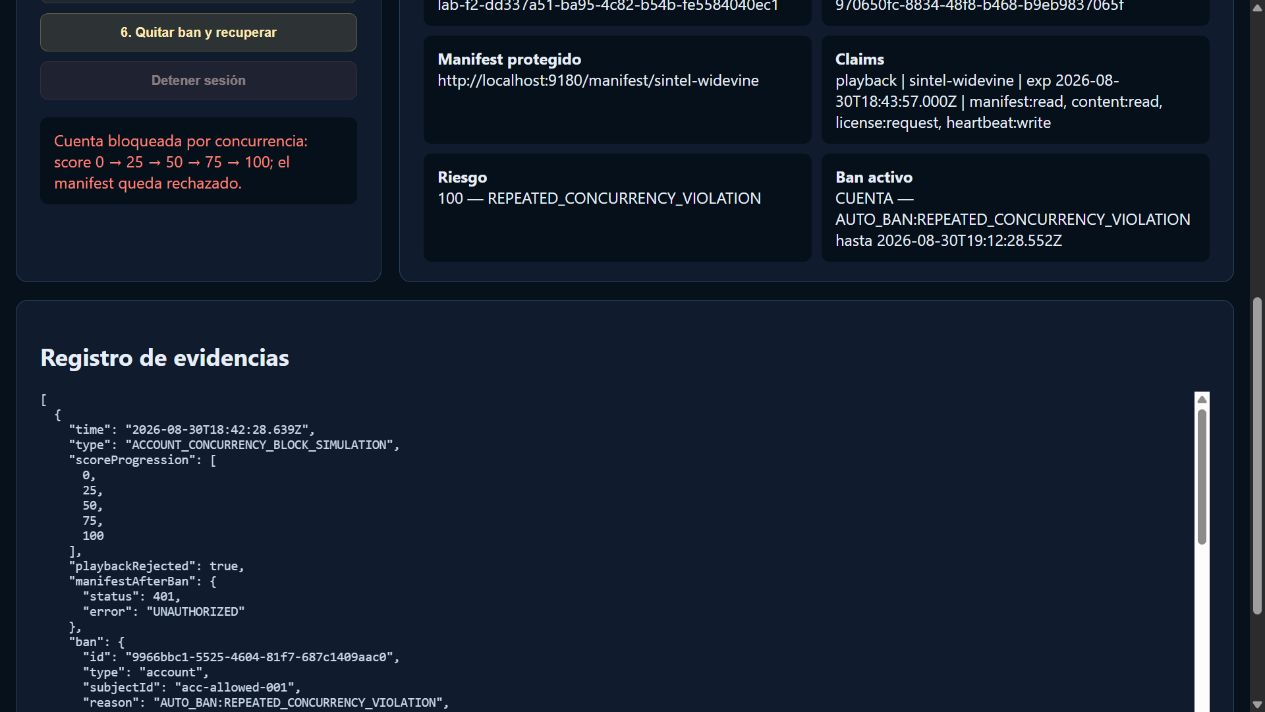
\includegraphics[width=0.98\textwidth]{figuras/fase2-laboratorio-bloqueo.png}
    \caption{Laboratorio de Fase~2 tras alcanzar 100 puntos por rechazos de concurrencia y activar el ban automático de cuenta.}
    \label{fig:fase2-laboratorio-bloqueo}
\end{figure}

La misma interfaz permite retirar cualquiera de los dos bans con el token administrativo y volver a reproducir. Para ello renueva la credencial mediante heartbeat o crea una nueva sesión si la anterior ha expirado durante el bloqueo. La retirada no reinicia el score, que permanece como rastro del comportamiento observado. Estas secuencias han proporcionado mecanismos controlados para el Capítulo~7, pero no han sustituido a las evidencias de red y servidor utilizadas para contrastar el resultado visible.

Se ha incorporado además un laboratorio específico de CDN leeching, accesible en \texttt{localhost:9302} y \texttt{localhost:9402}. Su backend actúa como un cliente externo no sujeto a CORS: autentica al usuario de prueba, crea una sesión y vuelve a servir al navegador el manifiesto y los segmentos obtenidos con la clave CENC conocida. La interfaz permite contrastar la ausencia de token, el origen web no permitido, una única reproducción válida, una segunda sesión, la copia del token desde otra instancia, el cruce de activo y el uso posterior a la parada. En Fase~2 muestra también el score y la razón generada al consumir contenido sin que se haya observado una solicitud de licencia. Las capturas y el análisis se presentan en el capítulo de evaluación.

\section{Integración completa del entorno}

El flujo integrado comienza en uno de los frontales web y converge en Varnish. Tras el login, el cliente conserva el token de acceso únicamente para crear sesiones y, en Fase~2, consultar administración. La sesión devuelve las URLs locales de manifiesto y licencia y un token efímero. Shaka Player introduce el contexto en sus filtros de red; el \textit{control-plane} valida y actualiza la sesión; y el servidor interno de licencia reenvía el challenge sin quedar expuesto al anfitrión. El laboratorio externo utiliza exactamente esas rutas, por lo que no dispone de un acceso privilegiado al origen.

En Fase~2, cada paso relevante produce además un evento y puede modificar el riesgo. La respuesta activa se aplica antes de alcanzar manifiesto, contenido, heartbeat o licencia. El plano administrativo permanece disponible para observar y revertir el estado. Redis se configura sin RDB ni AOF para que reiniciar el contenedor deje el laboratorio en un estado conocido; la persistencia duradera y la alta disponibilidad no forman parte de esta implementación.

Con esta integración han quedado implementadas las dos etapas de mejora: Fase~1 corrige los caminos de acceso y crea una sesión verificable; Fase~2 añade memoria del comportamiento y capacidad de bloqueo. En el Capítulo~7 se ha evaluado si estos mecanismos producen las respuestas esperadas frente a los escenarios de Fase~0, qué evidencias dejan y qué coste funcional introducen.
